\documentclass{standalone}
\begin{document}
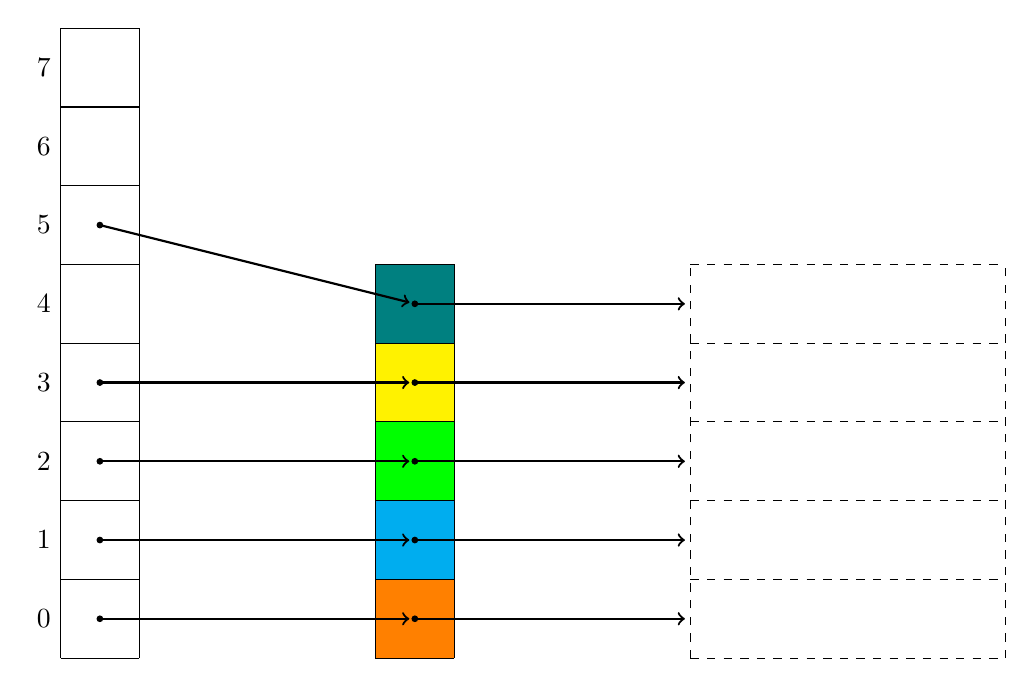
\begin{tikzpicture}

\fill[orange] (4, 0) rectangle (5, 1);
\fill[cyan] (4, 1) rectangle (5, 2);
\fill[green] (4, 2) rectangle (5, 3);
\fill[yellow] (4, 3) rectangle (5, 4);
\fill[teal] (4, 4) rectangle (5, 5);

\draw (1, 0) -- (1, 8);
\draw (0, 0) -- (0, 8);
\foreach \i in {0,...,8}
{
    \draw (0, \i) -- (1, \i);
}

\draw (0, 0.5) node[left]{$0$};
\draw (0, 1.5) node[left]{$1$};
\draw (0, 2.5) node[left]{$2$};
\draw (0, 3.5) node[left]{$3$};

\draw (0, 4.5) node[left]{$4$};
\draw (0, 5.5) node[left]{$5$};
\draw (0, 6.5) node[left]{$6$};
\draw (0, 7.5) node[left]{$7$};

\draw (4, 0) -- (4, 5);
\draw (5, 0) -- (5, 5);
\foreach \i in {0,...,5}
{
    \draw (4, \i) -- (5, \i);
}

\draw[thick,->,shorten >=2pt] (0.5, 0.5) -- (4.5, 0.5);
\draw[thick,->,shorten >=2pt] (0.5, 1.5) -- (4.5, 1.5);
\draw[thick,->,shorten >=2pt] (0.5, 2.5) -- (4.5, 2.5);
\draw[thick,->,shorten >=2pt] (0.5, 3.5) -- (4.5, 3.5);
\draw[thick,->,shorten >=2pt] (0.5, 5.5) -- (4.5, 4.5);
\draw[fill] (0.5, 0.5) circle (1pt);
\draw[fill] (0.5, 1.5) circle (1pt);
\draw[fill] (0.5, 2.5) circle (1pt);
\draw[fill] (0.5, 3.5) circle (1pt);
\draw[fill] (0.5, 5.5) circle (1pt);

    \draw[dashed] (8, 0) -- (8, 5);
    \draw[dashed] (12, 0) -- (12, 5);
\foreach \i in {0,...,5}
{
    \draw[dashed] (8, \i) -- (12, \i);
}

\draw[thick,->,shorten >=2pt] (4.5, 0.5) -- (8, 0.5);
\draw[thick,->,shorten >=2pt] (4.5, 1.5) -- (8, 1.5);
\draw[thick,->,shorten >=2pt] (4.5, 2.5) -- (8, 2.5);
\draw[thick,->,shorten >=2pt] (4.5, 3.5) -- (8, 3.5);
\draw[thick,->,shorten >=2pt] (4.5, 4.5) -- (8, 4.5);
\draw[fill] (4.5, 0.5) circle (1pt);
\draw[fill] (4.5, 1.5) circle (1pt);
\draw[fill] (4.5, 2.5) circle (1pt);
\draw[fill] (4.5, 3.5) circle (1pt);
\draw[fill] (4.5, 4.5) circle (1pt);



\end{tikzpicture}
\end{document}
